\documentclass [a4paper, 11pt] {article}

\newcommand\seancetitle{Implémentation Python}
\newcommand\seancenumber{4}
\def\AvecSolutions{}  % Commenter pour ne pas afficher les solutions

\usepackage[utf8]{inputenc}  
\usepackage[T1]{fontenc}  
\usepackage{lmodern}
\usepackage[french]{babel}
\usepackage{fancybox}
\usepackage{listings}
\usepackage{color}
\usepackage{tikz}
\usetikzlibrary{babel}
\usetikzlibrary{decorations.markings}
\usepackage{pgfplots}
\pgfplotsset{compat=1.18}
\pgfplotsset{samples=200}
\usepackage{graphicx,subfigure}
\usepackage[titletoc]{appendix}
\usepackage{float} % figures flottantes 
\usepackage{here} % figures flottantes
\usepackage{url}
\usepackage{enumitem}
\setlist[itemize]{label={$\bullet$}}
%\setlist[enumerate]{noitemsep, nolistsep}
\usepackage{xcolor}
\usepackage[colorlinks=true]{hyperref}
\usepackage{tabularx}
\usepackage{minted}
\usepackage{amsmath}
\usepackage[skins,breakable]{tcolorbox}
\usepackage{verbatim}
\usepackage[europeanresistors,siunitx]{circuitikz}
\usepackage{multicol}
\usepackage{physics}
\usepackage[outline]{contour} % glow around text
%\usetikzlibrary{intersections}
%\usetikzlibrary{decorations.markings}
\usetikzlibrary{angles,quotes} % for pic
\usetikzlibrary{bending} % for arrow head angle
\contourlength{1.0pt}
\usetikzlibrary{3d}
\usetikzlibrary{trees}
\usepackage{dirtytalk}

% --------------------------------------------------------------
% Title
% --------------------------------------------------------------
\makeatletter
\newcommand\maintitle[1]{
    \quitvmode
    \hb@xt@\linewidth{
        \dimen@=1ex
        \advance\dimen@-2pt
        \leaders\hrule \@height1ex \@depth-\dimen@\hfill
        \enskip
        \textbf{#1}
        \enskip
        \leaders\hrule \@height1ex \@depth-\dimen@\hfill
    }
}
\makeatother

\newcommand{\makeseancetitle}{
\begin{center}
    \Large
    \centering
    \maintitle{LELEC1930 - Introduction aux télécommunications}\\
    \textsc{\textbf{Séance \seancenumber{} - \seancetitle{}}}\\
    \vspace{0.1cm}
    \normalsize
    Prof. : Jérôme Louveaux \hfill Assist. : Jérome Eertmans\\
   \noindent\hrulefill
\end{center}
}

\newcommand{\makerappeltitle}{
\begin{center}
    \Large
    \centering
    \maintitle{LELEC1930 - Introduction aux télécommunications}\\
    \textsc{\textbf{Rappel - \seancetitle{}}}\\
    \vspace{0.1cm}
    \normalsize
    Prof. : Jérôme Louveaux \hfill Assist. : Jérome Eertmans\\
   \noindent\hrulefill
\end{center}
}

\usepackage{fancyhdr}
\fancypagestyle{firstpage}
{
   \cfoot{Page \thepage}
}
\fancypagestyle{nextpages}
{
    \lhead{Séance \seancenumber{}}
    \chead{\seancetitle}
    \rhead{LELEC1930}
    \cfoot{Page \thepage}
}
\fancypagestyle{rappelnextpages}
{
    \lhead{Rappel}
    \chead{\seancetitle}
    \rhead{LELEC1930}
    \cfoot{Page \thepage}
}

\setlength{\headheight}{13.59999pt}

% --------------------------------------------------------------
% Some parameters
% --------------------------------------------------------------
\oddsidemargin =0 mm
\topmargin = -10 mm
\footskip = 20mm
\textheight = 240 mm 
\textwidth = 160mm

% --------------------------------------------------------------
% Exercice environments
% --------------------------------------------------------------
\newcounter{exercice}

\definecolor{exercice_color}{RGB}{21,76,121}
\definecolor{exercice_color_fill}{RGB}{252,248,227}

\newcommand{\theexerciceref}{No reference}

\makeatletter
\newenvironment{exercice}[2][\texorpdfstring{\unskip}{}]
{
\refstepcounter{exercice}
\def\@currentlabel{{#2}}
\label{ref-exercice-\theexercice}
\addcontentsline{toc}{subsubsection}{{#2} #1}
\noindent
\flushleft
\begin{tikzpicture}
    \draw[very thick,exercice_color] (0,0) -- ++(0,+7.5pt)
    -- ++(\textwidth,0) node[midway,above] {\textbf{Exercice #2 : #1}}
    -- ++(0,-7.5pt);
\end{tikzpicture}
\vspace{-.3cm}
\begin{tcolorbox}[
    blanker,
    width=\textwidth,
    breakable]
}
{   \end{tcolorbox}
\vspace{-.4cm}
\flushleft
\begin{tikzpicture}
    \draw[very thick,exercice_color] (0,0) -- ++(0,-7.5pt)
    -- ++(\textwidth,0)
    -- ++(0,+7.5pt);
\end{tikzpicture}
}
\makeatother

\ifcsname AvecSolutions\endcsname
\newenvironment{reponse}
{
\noindent
\begin{tcolorbox}[
    colframe=exercice_color,
    colback=exercice_color_fill,
    coltitle=exercice_color_fill,  
    title=\centering\textbf{{\hypersetup{allcolors=white} Réponse à l'exercice \ref{ref-exercice-\theexercice} :}},
    breakable,
    width=\textwidth]
}
{   \end{tcolorbox}
}
\else
\newenvironment{reponse}{\comment}{\endcomment}
\fi


% --------------------------------------------------------------
% Code environments
% --------------------------------------------------------------
\usemintedstyle{borland}
\providecommand*{\listingautorefname}{Listing}

\newenvironment{python}
{\VerbatimEnvironment
\begin{minted}[
linenos,
% fontfamily=courier,
fontsize=\normalsize,
xleftmargin=21pt,
]{python}}
{\end{minted}}

\newcommand\py[1]{\mintinline{python}{#1}}

\newcommand\la[1]{\mintinline{latex}{#1}}

% Vertical line in matrices

\makeatletter
\renewcommand*\env@matrix[1][*\c@MaxMatrixCols c]{%
  \hskip -\arraycolsep
  \let\@ifnextchar\new@ifnextchar
  \array{#1}}
\makeatother

% Double underline
\def\doubleunderline#1{\underline{\underline{#1}}}


\begin{document}

    \makeseancetitle
    \thispagestyle{firstpage}
    
    \part*{Rappel}
    
    En télécommunications, la majorité, si pas l'entièreté, des calculs sont effectués sur un ordinateur. Le but de cette séance est donc de vous familiariser avec l'implémentation de concepts vus au cours à l'aide du langage de programmation \py{Python}.
    
    Afin de pouvoir mener à bien cette séance, on vous demandera d'\textbf{installer les packages} \py{numpy} et \py{scipy}. En plus de ces derniers, il vous est conseillé d'installer les packages \py{matplotlib} et \py{notebook}. Le premier permet de tracer des graphiques scientifiques très aisément, tandis que le second offre un environnement de programmation propice aux tests.
    
    En bref, vous pouvez tout installer via une seule commande dans votre terminal : \texttt{pip install numpy scipy matplotlib notebook}.
    
    \paragraph{Note :} \textit{La plupart de ces packages sont installés par défaut si vous utilisez Anaconda.}
    
    \begin{python}
import numpy as np
import matplotlib.pyplot as plt

# Exemple de plot

x = np.linspace(-5, 5, 25)  # 25 valeurs entre -5 et 5 (compris)
y = x ** 2

plt.plot(x, y)
plt.xlabel("x")
plt.ylabel("y")
plt.title("Une jolie parabole")
plt.show()  # Affiche le graphique, non nécessaire dans un Notebook
    \end{python}
    
    \begin{figure}[H]
        \centering
        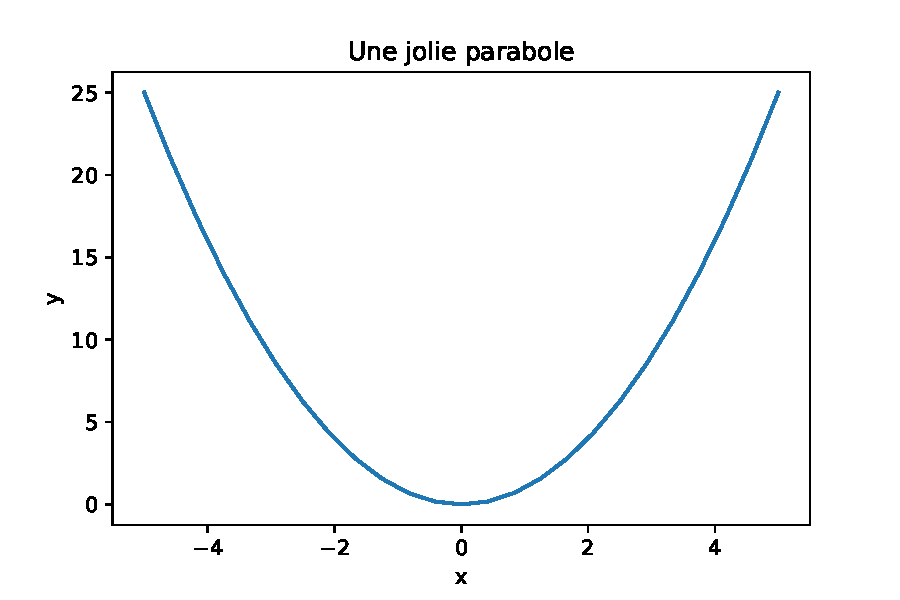
\includegraphics[width=0.5\textwidth]{imgs/parabole.pdf}
        \caption{Résultat obtenu avec le code ci-dessus.}
        \label{fig:parabole}
    \end{figure}
    
    Plus tout autre question concernant le code, ne l'oubliez jamais : Google est votre ami ! L'assistant aussi par ailleurs ;-)
    
    \pagebreak
    \pagestyle{nextpages}
    \part*{Exercices}
    
    \begin{exercice}[Calcul du BER d'un QAM-4]{1}
    
        L'objectif de cet exercice est de réussir à calculer le Bit Error Rate (BER), taux d'erreur en français, d'un signal et de voir son évolution en fonction du niveau de bruit, ou plutôt du Signal to Noise Ratio SNR.
        
        On considère donc la transmission d'une séquence de $N=\num{1e6}$ symboles QAM-4 :
        \begin{equation}
            x[k] = \pm 1 \pm j,
        \end{equation}
        avec $k=0,...,N$.
        
        Lors de l'envoi, le canal de transmission ajoute un bruit sur le signal de telle manière que le signal reçu, $y$, soit de la forme :
        \begin{equation}
            y[k] = x[k] + n[k],
        \end{equation}
        avec $n[k]$ le bruit à l'instant $k$.
        
        Ici, on modélise le bruit comme étant un bruit blanc gaussien, c.-à-.d une variable aléatoire suivant une distribution normale de moyenne nulle. Les symboles étant complexes, le bruit l'est tout autant. On notera donc $\sigma_n^2$ la variance du bruit complexe, et $\sigma_n^2/2$ la variance des parties réelles et imaginaires.
        
        Au récepteur, chaque symbole est décodé comme étant celui le plus proche de $y[k]$. On notera l'estimation du signal original $\hat{x}[k]$. Dans un monde idéal, sans bruit, on aura donc que $x[k]=\hat{x}[k]$ pour tout $k$. Le BER du signal est donc simplement le nombre de symboles erronés dans $\hat{x}[k]$ sur le nombre total de symboles.
        
        Finalement, on définit le SNR comme :
        \begin{equation}
            \text{SNR} = \frac{2}{\sigma_n^2}.
        \end{equation}
        
        \begin{enumerate}
            \item Générez la séquence $x[k]$ de manière aléatoire (voir \href{https://numpy.org/doc/stable/reference/random/generated/numpy.random.randint.html}{\py{numpy.random.randint}}).
            \item Générez la séquence $n[k]$ de bruit avec $\sigma_n^2 = \num{1e-2}$ (voir \href{https://numpy.org/doc/stable/reference/random/generated/numpy.random.randn.html}{\py{numpy.random.randn}}).
            \item Calculez les échantillons $y[k]$ et afficher les sur le diagramme de la constellation.
            \item Estimez le symbole d'origine $\hat{x}[k]$ sur base de cet échantillon.
            \item Calculez le BER.
            \item Refaites toutes ces étapes pour différents niveaux de bruits (conseil : utilisez \py{np.logspace(-2, 1, 25)}).
            \item Tracez la courbe du BER versus le SNR (conseil : utilisez \py{plt.semilogy(10 * np.log10(SNR), BER)}) et vérifiez que vous obtenez des résultats cohérents.
        \end{enumerate}
    
    \end{exercice}
    
    \begin{reponse}
        Une solution possible à l'exercice peut être visionnée dans ce \href{https://github.com/jeertmans/LELEC1930/blob/main/notebooks/seance4.ipynb}{Notebook}.
    \end{reponse}
    
    \begin{exercice}[Transformée en cosinus discrète]{2}
    
        La transformée en cosinus discrète (DCT) est opération mathématique sans perte qui permet d'exprimer un signal en fonction de son contenu fréquentiel. Similaire à la transformée de Fourier, la DCT est très utilisée lors de la compression d'images (exemple : JPEG).
        
        Ici, vous allez travailler avec des images de taille $8 \times 8$. Comme les images sont des matrices de pixels, et non de vecteurs, il faut appliquer deux fois la DCT : une fois pour les lignes, une fois pour les colonnes. On appellera cette fonction \py{dct2} et son inverse \py{idct2}. Pour une matrice $N\times N$, on définit la DCT2 de $X$ comme :
        
        \begin{equation}
            Y(u,v) = \frac{2 C(u) C(v)}{N} \sum\limits_{m=0}^{N-1}\sum\limits_{n=0}^{N-1} X(m,n) \cos\frac{(2m+1)u\pi}{2N})\cos\frac{(2v+1)v\pi}{2N},
        \end{equation}
        avec $C(0)=1/\sqrt{2}$ et $C(k) = 1$ pour $1 \le k \le N-1$.
    
        \begin{python}
import numpy as np
from scipy.fftpack import dct, idct

def dct2(X):
    return dct(dct(X.T, norm="ortho").T, norm="ortho")

def idct2(Y):
    return idct(idct(Y.T, norm="ortho").T, norm="ortho")

blocks = np.load("seance4.npy", allow_pickle=True).item()
        \end{python}
        
        Le code ci-dessus montre comment définir la DCT sur une matrice à partir de la DCT sur un vecteur. La variable \py{blocks} est un dictionnaire contenant toutes les matrices nécessaires à l'exercice. Vous trouverez le fichier \py{seance4.npy} sur Moodle.
        
        Pour finir, vous pouvez afficher le contenu d'une matrice de la manière suivante.
        
        \begin{python}
import matplotlib.pyplot as plt

def plot_image(X, ax=None):
    if ax is None:  # Si on ne fournit pas d'axes, on en crée
        _, ax = plt.subplots()

    im = ax.imshow(X, origin="lower")
    bar = plt.colorbar(im, ax=ax)

    ax.set_xlabel("m / u")
    ax.set_ylabel("n / v")
    bar.set_label("Valeur pixel")
        \end{python}
    
    \begin{enumerate}
        \item Observez les trois premiers blocs (\py{"img1"}, \py{"img2"} et \py{"img3"}) et calculez les valeurs de leurs coefficients DCT. Essayez d’interpréter les résultats.
        \item On observe que le coefficient principal est toujours non nul. À quoi correspond-il ? Que faudrait-il faire pour obtenir un coefficient principal nul ?
        \item Observez les blocs 4 et 5, qui sont définis entre -1 et 1, et leur DCT. Interprétez les résultats. Puis comparez avec le bloc 6 (défini entre 0 et 1).
        \item Observez les blocs 7 et 8, et tentez de prédire quels coefficients DCT seront majoritairement présents.
        \item Observez les valeurs du bloc 9, et tentez de prédire les valeurs exactes des coefficients DCT de celui-ci, à partir des résultats obtenus pour les blocs 1 et 3.
        \item Finalement, vous pouvez utiliser le bloc 10 pour faire un petit test de compression. La matrice \py{"Q"} fournie contient les coefficients de quantification habituels en JPEG. Ils sont calibrés pour des valeurs de pixels entre 0 et 256, vous utiliserez donc plutôt la matrice \py{Q2 = Q / 256}.
        \begin{enumerate}
            \item Appliquez la DCT sur le bloc 10.
            \item Appliquez la quantification en divisant les coefficients par ceux de \py{Q2}, puis arrondissez à l’entier le plus proche. Observez les coefficients restants.
            \item Retrouvez les coefficients compressés en re-multipliant par \py{Q2}, élément par élément.
            \item Appliquez la DCT inverse et observer la nouvelle image obtenue. Comparez-la en observant les deux images côte à côte.
            \item Vous pouvez également tester des quantifications plus ou moins fortes en multipliant toute la matrice \py{Q2} par une constante.
            \item Si le DCT est une transformation sans perte, pourquoi la compression JPEG, qui utilise la DCT, est-elle une transformation \textbf{avec perte} ?
        \end{enumerate}
    \end{enumerate}
    
    \end{exercice}
    
    \begin{reponse}
        Une solution possible à l'exercice peut être visionnée dans ce \href{https://github.com/jeertmans/LELEC1930/blob/main/notebooks/seance4.ipynb}{Notebook}.
    \end{reponse}

\end{document}